\chapter{Configuring Advanced Networking}

\section{Networking Basics Resumed}
\subsection{Network configuration tools}
\begin{tabular}{rM{0.68}}
	\toprule
	\textbf{Terms} &\textbf{Description} \\
	\midrule
	\textbf{ip addr show}	&Shows address information about all network interfaces.\\
	\midrule
	\textbf{ip -s link show ens33}	&Shows statistics about packets but for interface \verb|ens33|. Same as \verb|ip -s link|, but for a specific interface. \\
	\midrule
	\textbf{ip route}	&Shows routing information\\
	\midrule
	\textbf{traceroute / tracepath}	&For analysing a particular route or path.\\
	\midrule
	\textbf{netstat / ss}	&Analyse ports and services currently listening for incoming connections.\\
	\bottomrule
\end{tabular}

\subsection{Network Manager}
\textbf{NetworkManager} is used to both manage and monitor network settings. While the settings made with the IP tool act directly on the NICs, they're temporary and wiped with every boot or even bringing the interface down and up again. The network manager uses config scripts in \verb|/etc/sysconfig/network-scripts| to store our configs and use them after every boot. The settings can be managed using either \verb|nmcli| or \verb|nmtui|. The former is preferred for scripts while \verb|nmtui| is preferred for manual configs. 

\subsubsection{nmcli concepts}
\begin{itemize}
	\item A \textbf{device} or an \textbf{interface} is a network interface, corresponding to the hardware NIC (Network Interface Card). 
	\item A \textbf{connection} is a collection of configuration settings for a \textit{device}. 
	\item Multiple connections can exist for the same device, but since they operate on the same settings for the device, only one of them can be active. 
	\item All the connections (and some details) can be shown with the command \verb|nmcli con show|. 
	\item To show all the details for a particular connection, we have to use the command \verb|nmcli con show <interface name>| like \verb|nmcli con show wlo1| (where \textit{wlo1} is the name of the connection).
	\item To see the connection status for a device, we use \verb|nmcli dev status|. This shows us which devices are connected and which connection they're presently using. 
	\item To see the details of the actual NIC device, we use \verb|nmcli dev show <deviceName>|.
\end{itemize}

\subsection{Creating Network Interfaces with nmcli}
\vspace{-10pt}
To add a new connection using \verb|nmcli| that has the name \textit{dhcp} that auto-connects using dynamic IP on interface \textit{eno1}, we use:

\vspace{-15pt}
\begin{minted}{console}
# nmcli con add con-name "dhcp" type ethernet ifname eno1 
\end{minted}
\vspace{-10pt}	

\noindent
To add a new connection \textit{static} that uses a static ip that doesn't connect automatically, we use:

\vspace{-15pt}
\begin{minted}{console}
# nmcli con add con-name "static" type ethernet ifname eno1 autoconnect no ip4 192.168.122.102 gw4 192.168.122.1
\end{minted}
\vspace{-10pt}	

\noindent
Now, the available connections can be checked with \verb|nmcli dev status|. The we can connect the \textit{static} connection using \verb|nmcli con up static| and then switch back to the original connection \textit{dhcp} using \verb|nmcli con up dhcp|.

\subsection{Modifying Network Interfaces using nmcli}

To see the details of the \textit{static} connection, we use \verb|nmcli con show static|. Then, to add/modify the DNS server address for that connection, we use the \verb|con mod| keywords, which makes the command:

\vspace{-15pt}
\begin{minted}{console}
# nmcli con mod "static" ipv4.dns 192.168.122.1
\end{minted}
\vspace{-10pt}	

\noindent
Note that the modification requires the \verb|ipv4| keyword instead \verb|ip4|. To define a second IPv4 DNS for the \textit{static} connection, we use the \verb|+| symbol to denote that a new value for the item should be added and the old value shouldn't be overwritten. The command then becomes: 

\vspace{-15pt}
\begin{minted}{console}
# nmcli con mod "static" +ipv4.dns 8.8.8.8
\end{minted}
\vspace{-10pt}	

\noindent
An existing static IP address and gateway can be edited using:

\vspace{-15pt}
\begin{minted}{console}
# nmcli con mod "static" ipv4.addresses "192.168.100.10/24 192.168.100.1"
\end{minted}
\vspace{-10pt}	

\noindent
A secondary IPv4 address can be added using:

\vspace{-15pt}
\begin{minted}{console}
# nmcli con mod "static" +ipv4.addresses "10.0.0.10/24"
\end{minted}
\vspace{-10pt}	

\noindent
Finally, to activate all the above settings, we use: \verb|nmcli con up static|.

\subsection{Working directly with Configuration Files}
All the \verb|nmcli| tool really does while adding or modifying settings is write the changes to the configuration files in \verb|/etc/sysconfig/network-scripts/ifcfg-<interfaceName>|. We may choose to edit them directly if needed. Then, after making the necessary modifications, we ask the NetworkManager service to reload the configuration using \verb|nmcli con reload|.

\subsection{Managing Hostname and DNS}
The hostname is stored in the file \verb|/etc/hostname| and can be edited directly or using the \verb|hostnamectl set-hostname <newHostName>| command. The current hostname can then be viewed using \verb|hostnamectl status|.

The value of the search domain and preferred nameserver (i.e., the one that the NetworkManager uses by default) is auto-pushed from \verb|/etc/sysconfif/network-scripts/|\\\verb|ifcfg-<connectionName>| to the file \verb|/etc/resolv.conf|. 

\section{Understanding Routing}
Let us consider the following network:

\begin{figure}[H]
	\centering
	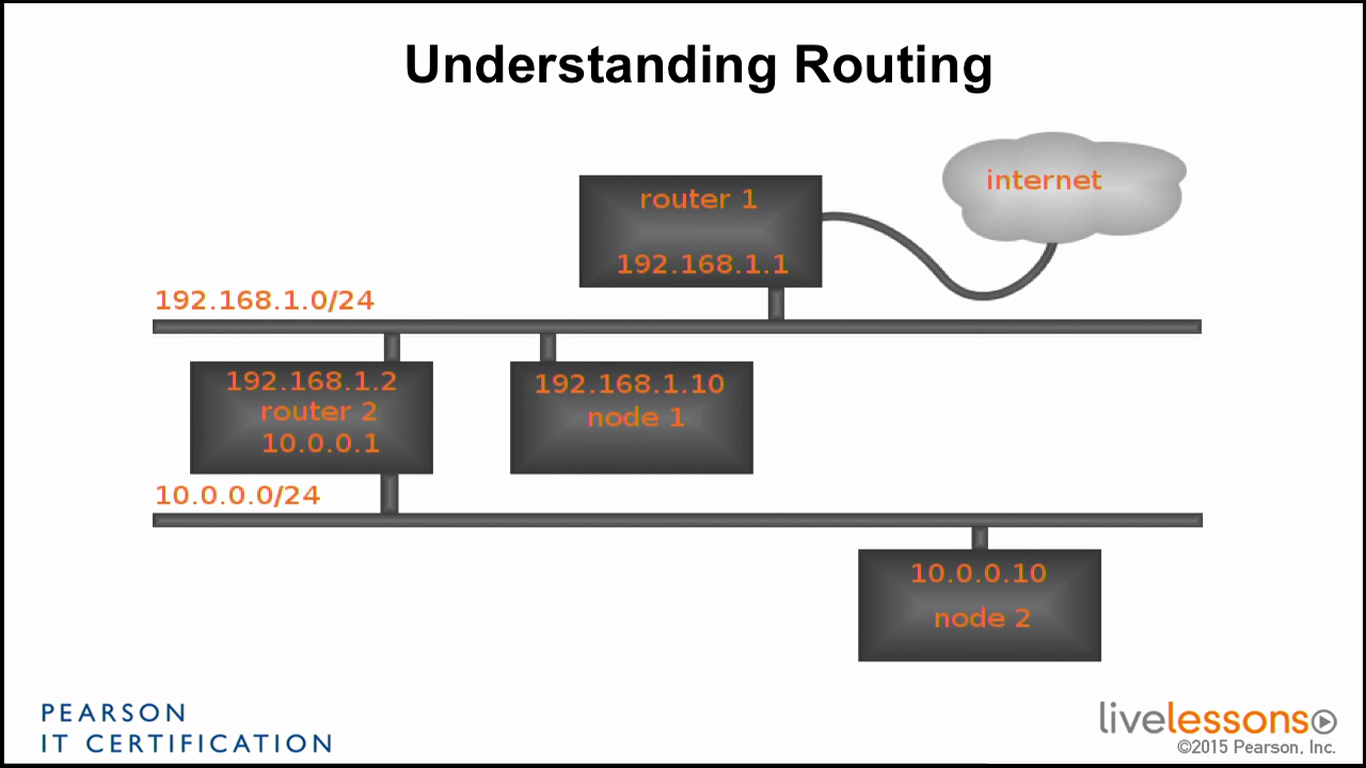
\includegraphics[width=0.9\linewidth]{Mod2/chapters/2.6.a}
	\caption{Sample Network}
	\label{fig:2}
\end{figure}

\noindent
Here, we see two different networks - the \verb|10.0.0.0/24| network connected to the inner \verb|192.168.1.0/24| network via \textit{router 2} (\verb|10.0.0.1|), which in turn connects to the internet via the edge router with IP \verb|192.168.1.1| - \textit{router 1}. 

For any packet headed to the internet on network 2, i.e., any packet originating from \textit{node 2}, the default gateway will have to be \textit{router 2} (\verb|10.0.0.1|). This gets the packet on to the \verb|192.168.1.0/24| network, where the default gateway is \textit{router 1} (\verb|192.168.1.1|), which passes it on to the internet. 

However, when the packets originate from node 1 (\verb|192.168.1.10|), there are two possible routes - if the packet is destined for the \verb|10.0.0.0/24| network, then the gateway should be \textit{router 2} (\verb|192.168.1.2|). But if the packet is for any other network, then the default gateway of \textit{router 1} (\verb|192.168.1.1|) should be used. Thus, a static route should be defined on node 1 for the \verb|10.0.0.0/24| network. 

\section{Setting up Static Routing}
The most convenient way to set up static routes is to use \verb|nmtui|. Let's assume we're setting up static routing for node 2 in our last example.

\begin{figure}[H]
	\centering
	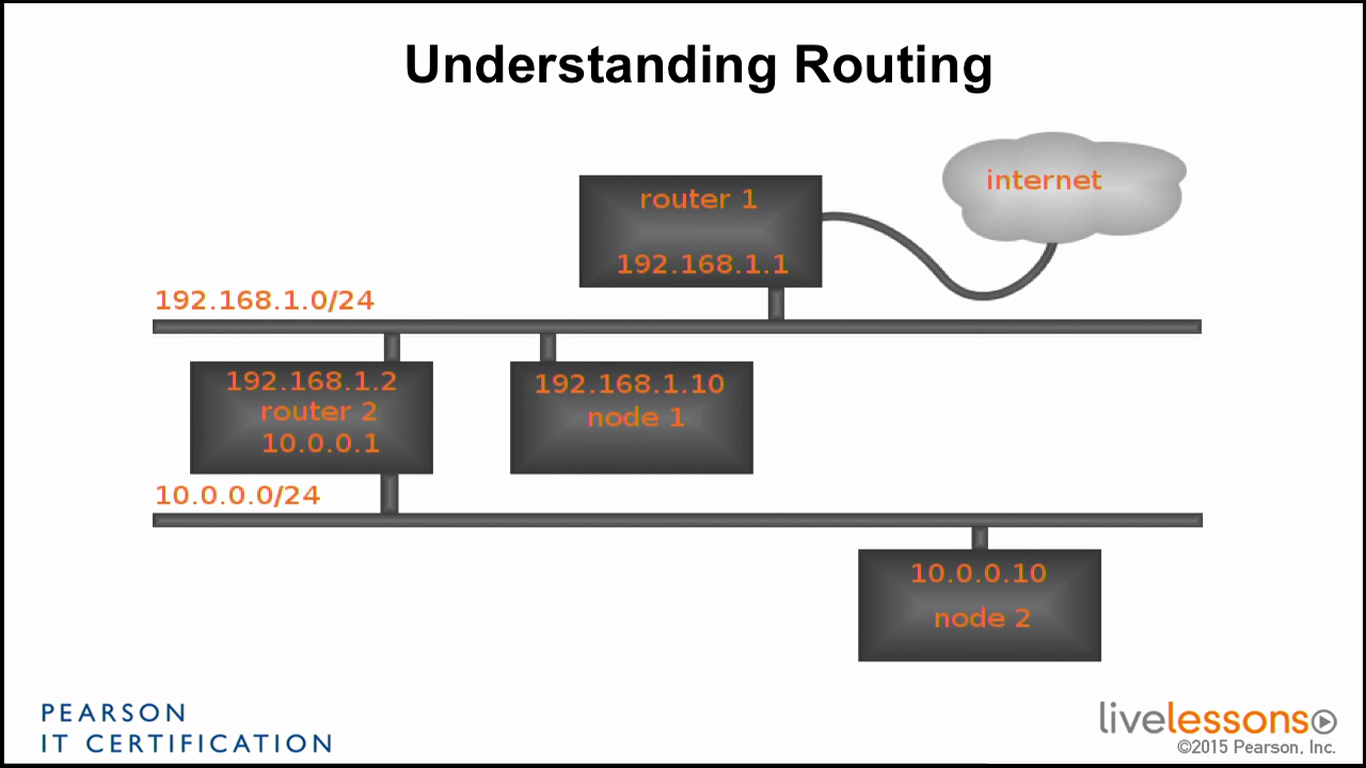
\includegraphics[width=0.9\linewidth]{Mod2/chapters/2.6.a}
	\caption{Network Diagram}
	\label{fig:2}
\end{figure}	

We need to edit the existing connection to include the new static route. For this, we select the options: \verb|Edit a Connection| $\rightarrow$ Select the connection to use $\rightarrow$ \verb|Edit...| $\rightarrow$ \verb|Routing| section $\rightarrow$ \verb|Edit...| $\rightarrow$ \verb|Add...| $\rightarrow$ Type the address of the network for which the static route will be defined in \verb|Destination/Prefix| (with the Network ID and prefix, like, \verb|10.0.0.0/24|) $\rightarrow$ Add the IP address of the router that leads to the network in the \verb|Next Hop| section (\verb|192.168.1.2| in our case). 

The \textbf{metric} of the connection is how a router chooses which route to take when there are multiple routes available to another network. Thus, it's only useful when there are multiple routes available for the same network, and is irrelevant to us right now. We now choose \verb|<Ok>| $\rightarrow$ \verb|<Ok>| $\rightarrow$ \verb|<Quit>|. 

Note however, that the new route won't be added to the network configuration till either the connection is \textit{refreshed} (by reactivating the connection) or the NetworkManager service is restarted. We could do this by \verb|nmtui| $\rightarrow$ \verb|Activate a Connection| $\rightarrow$ Select the connection which we edited $\rightarrow$ \verb|Activate|. Now the output of \verb|ip route show| will show the static route as well. 

If the interface name was \textit{ens33}, The \verb|/etc/sysconfig/network-scripts| directory now has a new file called : \verb|route-ens33| with the following contents:

\vspace{-15pt}
\begin{minted}{bash}
ADDRESS0=10.0.0.0
NETMASK0=255.255.255.0
GATEWAY0=192.168.1.2
\end{minted}
\vspace{-10pt}	

\noindent
Note that the nmtui utility has translated the \verb|/24| prefix from the \textbf{CIDR} (Classless Inter-Domain Routing) notation \verb|10.0.0.0/24| to the standard Network IP and Network Masks, where \verb|/24| translates to the network mask of \verb|255.255.255.0|. 